% !Mode:: "TeX:UTF-8"
\newcommand{\specialcell}[2][c]{%
  \begin{tabular}[#1]{@{}c@{}}#2\end{tabular}}
\newcommand{\mthead}[1]{\textit{\textbf{#1}}}

\newcommand{\newmodel}[1]{\textbf{#1.}\cite{#1}\quad}

\chapter{绪论}[Introduction]

\section{背景}[Background]

虽然目前很多公司都开发了自己的自动驾驶系统,但其使用的技术几乎都是基于计算机视觉,目标检测,目标识别等深度学习、机器学习技术。因此,针对自动驾驶系统的测试技术也是源于深度学习系统的测试技术。其中,在基于深度神经网络的自动驾驶系统中,其神经网络模型将被汽车的各种传感器(雷达、摄像头等)接收到的数据作为输入,经过其控制系统,通常为深度神经网络,的运算处理后输出各种驾驶行为(方向盘拐角、刹车信号,速度控制信号等)。下图\ref{as_example}展示了一个基于卷积神经网络的自动驾驶系统例子,这个系统由输入(摄像头拍摄的图像)、输出层(方向盘拐角)和中间的隐藏层组成。本章主要讲述传统的深度学习测试技术以及目前学术界比较推崇的自动测试技术。

\begin{figure}[h]
    \centering
    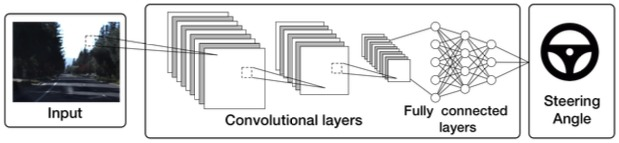
\includegraphics[width=0.8\textwidth]{as_example}
    \caption{基于卷积神经网络的自动驾驶系统\cite{DeepRoad}}
    \label{as_example}
\end{figure}

\subsection{传统的深度学习系统测试技术}[The traditional testing technology of DNN]

深度神经网络,通常指一个元组$N=(L,T,\Theta)$,这里$L=\{L_k|k\in \{1..K\}\}$代表一组网络层,$T\subseteq L\times L$代表各层之间的连接组合,$\Theta=\{\theta_k|k\in \{2,...,K\}\}$代表一组函数,每个函数代表非输入层的激活函数。在一个深度神经网络中,$L_1$指输入层,$L_K$指输出层,其他的层叫做隐藏层。每一层$L_k$由$s_k$个神经元组成,$k$层的第$l$个神经元记为$n_{k,l}$,每个神经元$n_{k,l},1\lt k \lt K, 1\leq l\leq s_k$跟两个变量相关$u_{k,l}$和$v_{k,l}$,分别表示神经元在经过激活函数处理前后的值。目前ReLU\cite{relu}函数是用在深度神经网络中当前最流行的激活函数,根据该函数隐藏层中的每个神经元的激活值可以定义为
\begin{gather}
    v_{k,l}=ReLU(u_{k,l})=\begin{cases}
        u_{k,l} & if\quad u_{k,l} \geq 0 \\
        0 & otherwise
    \end{cases}
\end{gather}
每个输入节点$n_{1,l}\leql 1 \leq s_1$都跟一个变量$v_{1,l}$有关,每个输出节点$n_{K,l},1\leq \leq s_K$跟变量$u_{K,l}$相关,因为已经没有激活函数可以作用在它们身上了。 

除了输入节点,其它的神经元都通过特定的参数跟下一层中的神经元相连接,令所有$k$和$l$都满足$2\leq k \leq K, 1\leq l \leq s_k$,则有
\begin{gather}
u_{k,l}=b_{k,l}+\sum_{1\leq h\leq s_{k-1}}w_{k-1,h,l}\dot v_{k-1,h}
\end{gather} 
这里$w_{k-1,h,l}$为$n_{k-1,h}$和$n_{k,l}$之间连接的权值,$b_{k,l}$称作神经元$n_{k,l}$的偏执项。这个定义可以表示全连接函数和卷积函数。函数$\theta_k$是上面两个公式的组合。得益于ReLU函数的使用,神经网络表现的行为是高度非线性的。

最后,对于任意输入,深度神经网络都有一个对应的标记,即对于该输入,输出层中拥有最大值的神经元下标:$label=\max_{1\leq l\leq s_K}u_{K,l}$。令$L$为标记的集合。

下图\ref{fig:dnn}为一个4层神经网络的例子,它的输入空间是$D_{L_1}=\mathbb{R}^2$,这里$\mathbb{R}$指整个实数集。
\begin{figure}[h]
    \centering
    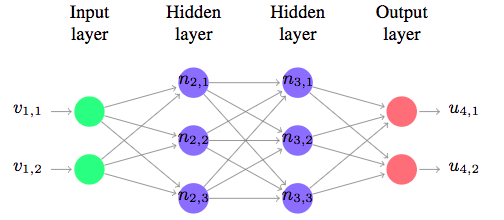
\includegraphics[width=.6\textwidth]{dnn_4}
    \caption{一个4层神经网络}
    \label{fig:dnn}
\end{figure}

深度学习技术是一种通过研究同类大量数据的表征,对未知新数据的特征进行推测的一门技术。在其行使职能,即预测新数据特征前,必须要学习大量同类的数据,即模型训练。模型训练完成后为了提前检测模型的准确性,会在之前的训练数据集中保留一部分数据,作为训练结束后的模型的测试数据集,使其在未被学习过的测试数据集上进行预测,最后以测试数据集上的准确性作为训练好的模型的精准度。目前学术界公认理想的训练数据集与测试数据集占比分别为70\%和30\%\cite{cs231n}。

其训练过程通常是以神经元为基本单位的神经网络为基本架构,采用向后传播算法来自动学习调节网络中的权值参数,训练过程中对权值初始数值的设置以及其他的初始训练参数的设置也十分重要,如果设置不当会有梯度消失,收敛时间过长等问题,当然训练数据集对训练结果的影响也很大。数据集的具体数量跟模型处理的具体问题相关,一般来说,处理的问题越复杂,即数据的特征越多,需要的数据量也就越多,比如比较出名的ImageNet\cite{ImageNet}比赛,公开可用的数据集多达1500万张由人工标注的图片数据。对于自动驾驶,也有诸多开源数据集,比如Oxford RobotCar\cite{ds:oxford},Comma.ai\cite{ds:ai},Udacity\cite{udacity_dataset},Berkeley大规模自动驾驶视频数据集\cite{ds:berkeley},Cityscape\cite{Cordts2016Cityscapes}等。深度学习技术对已有数据特征拟合的本质和其训练测试的过程导致其对数据量的严重依赖,传统的深度学习测试需要大量的人工收集、标注数据,着极度的增加了其中的人力成本。除此之外,传统的通过人工收集数据的方式有严重的缺点,即收集到的数据无法保证覆盖到了所有可能的极端场景,以自动驾驶测试数据集为例,人工收集的数据集一般是车载记录仪记录的道路驾驶视频图片,但一般大雨、大雪等极端天气场景数据很少也很难收集,这就给相应的极端场景自动驾驶系统测试带来了不确定性。 

\subsection{针对深度学习和自动驾驶的软件测试研究}

针对上诉问题,学术界提出了DeepXplore,在此其基础上,针对自动驾驶的软件测试,进一步提出了DeepTest和DeepRoad实现了深度学习系统测试用例自动生成系统来缓解深度学习系统对于数据量的依赖。除此外,针对训练数据集数量可能不够等问题,还有DeepMutation\cite{DeepMutation}、DeepCover\cite{DeepCover}等工作被提出。下面对以上几项针对深度学习和自动驾驶系统的软件测试技术和传统的软件测试做一个简单的介绍。

\subsubsection{传统的软件测试技术}

传统的软件测试方法可粗略地分为黑盒测试和白盒测试两大类。黑盒测试主要针对测试软件的功能是否如预期运作,而不关心软件内部逻辑结构的运行是否合理等。测试者将软件当做一个黑箱,只指定输入,然后观察软件的输出是否正确。白盒测试则与黑盒测试相反,它主要关心的是程序软件内部逻辑是否运行如预期,重点测试软件内部的部件功能,是基于系统内部部件行为分析的测试方法,常常被用在单元测试和集成测试中。除此外,在传统的软件测试技术中还有一个重要的指标:测试/代码覆盖率,该指标常被用来描述当程序运行一个特定的测试用例时,程序里被执行到的代码部分,通常以百分比的形式表示,测试用例有较高的代码覆盖率的程序存在BUG的概率会小于代码覆盖率低的程序。下面讲到的现主流深度学习测试技术多数属于白盒测试的范畴。

\subsubsection{DeepXplore}[DeepXplore]
DeepXplore首先指出了深度学习系统与传统的软件开发系统的不同:传统软件的开发人员直接指定软件系统的逻辑,然而深度学习则是从数据特征中“学习、推到”它们的运行规则,甚至对于深度学习系统的开发人员来说,他们都不一定清楚训练好的深度学习模型的确切运行逻辑。因此DeepXplore
不是直接寻找深度学习系统中的逻辑错误,而是通过自动产生、寻找一些能使多个同类深度学习系统做出不同行为判断的测试用例,并通过这些触发被测试的DNN系统针对同一测试用例产生不同行为判断的行为推测出被测试系统中必有一个或多个系统存在BUG行为,然后并将这些找到的测试用例放回原训练数据集里重新训练模型,试图修正之前错误的行为。

\begin{algorithm}[ht]
    \small
    \SetAlgoLined
    \SetKwInOut{Input}{Input}
    \SetKwInOut{Output}{Output}
    \SetKwInOut{Variable}{Variable}

    \Input{Transformations T, Seed Images I}
    \Output{Generated Test Cases}
    \Variable{S: Stack to save outputs; Tqueue: Queue to save transformations}

    push all seed imgs to Stack S;\;
    $genTests = \varnothing$\;
    \While{S is not empty}{
        img = S.pop()\;
        $Tqueue = \varnothing$\;
        numFailedTries = 0 \;
        \While{$numFailedTries \leq maxFailedTries$}{
            \eIf{$Tqueue\ is\ not\ empty$}{
                T1 = Tqueue.deque()
            }{
                Randomly pick transformations T1 from T
            }
            Randomly pick parameter P1 for T1\;
            Randomly pick transformation T2 from T\;
            Randomly pick parameter P2 from T2\;
            newImage = ApplyTransforms(image, T1, P1m T2, P2)\;
            \eIf{covInc(newiamge)}{
                Tqueue.enqueue(T1)
                Tqueue.enqueue(T2)
                UpdateCoverage()
                $genTests=genTests \cup newiamge S.push(newImage)$
            }{
                $numFailedTries=numFailed++$
            }
        }
    }
    return genTests
    \caption{混合变换优化算法\cite{DeepTest}}
    \label{alg1}
\end{algorithm}

除了将使不同的DNN系统做出不同预测行为为目标外,DeepXplore也借鉴了传统软件测试技术中的代码覆盖率的概念,为了使得尽可能测试整个DNN系统,DeepXplore引入了神经元覆盖率的概念,即测试用例测试过程中,在整个深度学习系统中,被“激活”,即输出值超过了某个阀值的神经元的个数占整个网络结构神经元总数的占比。与代码覆盖率类似,我们期望神经元覆盖率越高越好。

DeepXplore以神经元覆盖率和使得不同DNN系统输出不一致为目标,将在原始测试用例上的修改抽象成为一个优化算法,使用梯度上升算法,最后自动生成一些使得被测的DNN系统得到不同的预测值,且各个DNN系统的神经元覆盖率很高的测试用例,DeepTest基于DeepXplore的工作,提出了一套专门针对自动驾驶系统,能够自动检测出错误行为的测试系统。发生在自动驾驶系统上的车祸大部分都是发生在一些罕见的路况场景下,而传统的自动驾驶检测测试技术几乎是完全依赖大量的罕见路况场景图片的人工收集与标注,这不仅包含了大量的人工成本,重要的是人工收集的数据无法保证能够覆盖度到了所有的极端场景数据。这些极端场景就好像是传统软件中的BUG,但是这些BUG一旦被检测到,就可能通过把这些导致错误的输入重新放入训练集,同时改变一下模型的结构和参数来修复。DeepTest正是通过以上的思路来设计的一套自动测试系统。

具体的实现上,DeepTest依旧借用DeepXplore提出的神经元覆盖率的概念,使用位移、拉伸、仿射以及直接修改像素的透明度等基本的图形变换的手段来合成新的驾驶图像,文章里提到合成后的数据能使原DNN系统的神经元覆盖率提升100\%\cite{DeepTest},并以提升神经元覆盖率为目标,给出了一个优化算法\ref{alg1},以获得最佳的图像混合变换,最后DeepTest在利用这些合成的新数据重新训练自动驾驶模型来提高模型对于极端场景的鲁棒性。

\subsubsection{DeepRoad}[DeepRoad]

尽管DeepTest已经提出了一个较为完善的自动驾驶系统测试方案,以相对便宜和简洁的方法,利用大量的原始和合成出来的驾驶场景图片成功地检测出了许多自动驾驶系统前后不一致的驾驶行为,但它有一个很严重的缺陷:DeepTest用来合成图片的技术很难合成一些能够精确反映现实驾驶场景的图片,并且现实驾驶场景的图片也很难由一些基础的仿射、位移变换模拟合成出来,其用来模拟雨天、雾天的场景的技术仅仅是在原始图层上添加一层额外的图层,如下图\ref{label-deeptest}所示,对于雾天,DeepTest仅仅是加了一层白色的图层,对于雨天,加了一层线条层。很明显这些合成图离现实中真实的驾驶场景有较大的差别。从另一个角度来说,即使用这些图检测出了自动驾驶系统错误的驾驶行为也很难有说服力,因为这些“出错”的场景在现实中根本不会出现。其实很多可能的真实的驾驶场景根本不能用一些简单的图像处理技术来模拟合成。

\begin{figure}[h]
    \centering
    \subfigure[DeepTest]{
        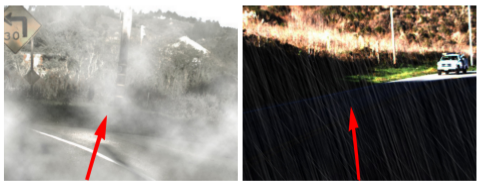
\includegraphics[width = 0.7\textwidth]{deeptest_effect}
    }
    \subfigure[DeepRoad]{
        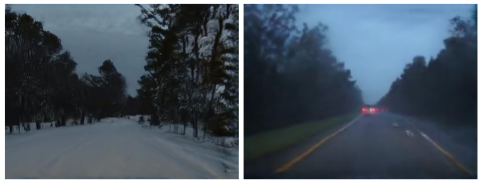
\includegraphics[width = 0.7\textwidth]{deeproad_effect}
    }
    \caption{天气场景合成效果图比较}
    \label{label-deeptest}
\end{figure}

为了能够自动地合成大量真实的驾驶场景图片,DeepRoad提出了一个半监督合成的框架,抛弃了DeepTest用到的简单的图像处理技术来合成图像,采用深度学习对抗生成网络的技术来合成相对较真实的驾驶场景图片,下图\ref{label-deeptest}为DeepTest合成图和DeepRoad使用对抗生成网络中UNIT\cite{UNIT}框架合成图的效果对比,其中图a红色箭头为自动驾驶系统对该驾驶场景输出的方向盘拐角。可以清楚的看到使用UNIT技术合成的效果比较好的驾驶场景图已经与真实场景很接近了。

DeepRoad将两种天气情况下的图片作为训练输入数据集,训练无监督对抗生成网络UNIT\cite{UNIT}框架,然后利用训练好的UNIT框架对未知新的输入数据进行转换合成,最后测试自动驾驶系统对使用UNIT进行转换后的图片做出的驾驶行为与未转换之前的原始图片的驾驶行为是否一致。

\subsubsection{DeepMutation}

深度学习系统的训练过程决定了其内部的系统逻辑很大程度上由其训练数据集决定,评价深度学习系统模型的标准方法是检测其在测试数据集上的性能水平。因此测试数据集的质量对于我们对模型的信任度至关重要。在数量不够的测试集即使上取得了高准确率,也缺少一般性和鲁棒性。在传统软件测试中,变异测试(Mutation Testing)对于评估测试集质量是一个相当成熟的技术,但是由于深度学习系统和传统软件的本质上的差异使得变异测试无法直接应用于深度学习软件系统中。DeepMutation提出了一个专门针对深度学习系统,评估其测试数据集质量的框架。它借用变异测试中本质思想,首先定义了一套源码级的变异操作子,对深度学习系统软件源码注入错误。进一步地,设计了一套模型级的变异操作子,比如对模型的神经网络层数进行增删操作,以及对单层网络的神经元进行增删操作,无须训练过程直接对深度学习系统注入错误。最终,测试数据集的质量可以根据注入的错误能被多大程度的检测出来分析得出。

\subsubsection{DeepCover}

传统的软件测试通过设置诸如代码覆盖率等指标来指示测试数据集的自动生成方向,但由于深度神经网络系统缺少类似传统软件的结构和逻辑控制流,因此如何为它们定义譬如分支覆盖率的指标并没有一个十分明显的方向。DeepCover\cite{DeepCover}对于深度神经网络系统提出了一个白盒测试方法,其中包含了一套测试覆盖指标和测试用例生成算法,即利用线性规划,通过扰动给定的测试用例来合成新的测试用例,弥补了传统软件和深度神经网络系统在这一方面的差异。

\subsubsection{NeVer}

NeVer\cite{dsv}提出了一个方法来验证神经网络系统安全性能。它主要关注的是多层神经元网络结构,定义了给定对于任意给定的输入值,其网络输出都保证在已知的范围内,则视该网络为“安全的”。进而NeVer还提出了一套启发式修复算法,能够自动提高测试的神经网络系统安全性能。

\subsection{其他的图像转换技术}[Other Image Transformation Technologies]

DeepRoad提出的将深度学习技术运用到自动驾驶系统测试用例合成,并设计的一套自动测试的框架在检测自动驾驶系统的稳定性和鲁棒性上,在其实验检测出了大量的现实自动驾驶系统有误的驾驶行为的结果\cite{DeepRoad}上看是有效的。其相对前人的工作DeepTest主要的改进是将测试用例的合成技术,即驾驶场景的图像转换技术,由原有的基本的图像变换换成了深度学习中的对抗生成网络技术。我们在利用UNIT合成驾驶场景图的实验过程中发现,虽然有效果比较好的合成图,但其占总的合成图的比例很小,1万张结果图中比较真实的图像大约有30多张,大部分的结果图如下,可以看到效果比较差,我们分析了效果比较差的原因主要是使用的训练数据集是由我们从Youtube上爬取的视频制作的数据图像,与UNIT官方使用的NVIDIA公司提供的闭源数据集相差比较大导致。

但其实目前学术界和工业界已经提出的能够进行不同天气场景图像转换的深度学习技术有很多。对此我们进行了调研,发现主要有两大类:对抗生成网络和图像风格转换(Neural Style Transfer)。以上两类技术的实现都是利用了神经网络的架构,这也是目前这类技术的主流模式。但除此之外还有很多没有使用诸如卷积神经网络架构的图像风格转换技术。这里有代表性的技术由基于笔画、线条进行渲染的技术。通常指通过一个对只有线条的画进行处理,最终渲染合成出一张具有某种风格的图像。这类算法的主要目的是根据有限的信息合成一张具有特定风格的图像。基于样例的渲染技术也属于没有采用神经网络架构实现图像合成的技术,这类算法通常会根据已有数据学习源数据到目标风格图片之间的映射函数,然后根据学习到的函数通过监督学习的方式将输入图片转换到目标风格图像空间上,从而实现图像的风格转换。

我们对DeepRoad进行的实验也表明在得不到理想的训练数据集的情况下利用UNIT进行图像转换的实验结果是不理想的,那么可否将UNIT更换为其他的能够进行图像转换的深度学习技术?哪一种技术的实现效果是最好的?如何评价各种图像转换技术在合成驾驶场景图上的好坏?哪一种技术的训练成本和实现成本是最小的?针对以上问题,我们对现有的能够实现图像风格转换的深度学习技术展开实证研究,希望能够找到答案,最终可以为以后的自动驾驶系统测试人员在选择驾驶场景图片测试用例的合成技术框架上提供一些有帮助的建议。

% TODO UNIT图像

\section{自动驾驶技术的发展}

本小节简要介绍自动驾驶技术的发展历程。

涉及自动驾驶技术的最早实验起始于1925年\cite{auto-driving-history}。在美国纽约,一辆名为“American Wonder”的无线电控制汽车从百老汇大姐驶过第五大道,它通过无线电接收器接受来自另一辆载人,并发出无线电信号的车辆引导行驶。自动引导驾驶行为的驾驶技术最早出现于1939年的万国博览会上,展出了一辆同样无线电控制汽车,由内嵌在公路里的芯片提供的电磁信场进而驱动车辆行驶。1958年,General Motors在此基础上提出了改进方案,在汽车的前部添加了能够检测到流过内嵌在公路内线路电流的电线圈,该电流可以被人为控制,进而影响汽车的方向盘转向。1977年,日本在此方案上作了进一步的改进,他们使用了一套能够将路况图像数据传输到计算机处理的摄影系统,但是装备了这套系统的车辆在当时最高时速只有20公里。10年后德国人同样使用了名为VaMoRs的摄影影像系统,并将汽车的最高时速提升到了56公里。 

\begin{figure}[ht]
    \centering
    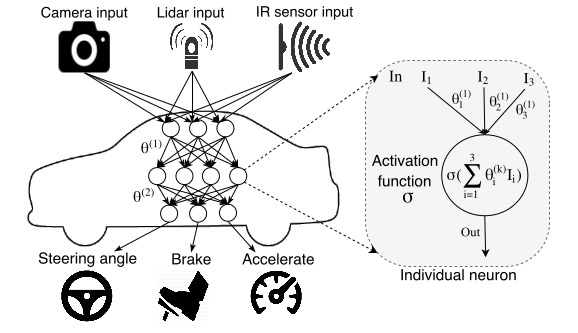
\includegraphics[width=0.8\textwidth]{auto-driving-sys}
    \caption{基于深度学习的自动驾驶系统}
    \label{auto-driving-sys}
\end{figure}

近年来,得益于深度学习技术的发展,基于深度学习的自动驾驶系统在对环境的感知和应对能力上也取得了许多突破,如上图\ref{auto-driving-sys}所示,目前的自动驾驶系统大致课分为3个部分,分别是负责接受外界数据的传感器单元,一般由摄像头、雷达和红外探测器组成。第二部分是系统的控制单元,它一般由多个神经元构成的多层神经网络组成,主要负责处理传感器接受的数据,利用诸如计算机视觉,物体检测,物体追踪等深度学习技术,最终输出一系列汽车控制信号,比如方向盘拐角信号、汽车油门信号和刹车信号等,达到汽车控制的目的。最后是汽车的实体功能单元。在本论文中,针对自动驾驶系统控制单元的研究,我们主要关注的输入是摄像头拍摄的路况图片,输出主要关注方向盘拐角信号。目前国内外许多公司开发的自动驾驶系统,比如Google公司的Waymo,Baidu公司的Apollo以及Tesla公司的Autopilot都是基于此类架构。

\section{自动驾驶系统测试技术国内外研究现状}

Pei K\cite{DeepXplore}等人首次针对自动驾驶系统测试,提出一个自动测试系统DeepXplore,基于已有的测试数据集自动生成新的,能够使测试的深度学习系统“出错”的测试用例,在深度学习系统测试用例自动生成框架领域具有里程碑的意义。时隔一年,Pei K同组的人基于DeepXplore的工作继续提出了DeepTest\cite{DeepTest}框架,其去掉了DeepXplore框架必须提供多个类似功能的深度学习系统的要求,同时针对自动驾驶系统测试用例的自动生成做了许多改动。至此,相对之前的深度学习测试技术来说,一个代价低廉,有效的测试系统框架基本行程。虽然文献\cite{DeepTest}将自动驾驶系统测试列为了DeepTest的使用场景之一,但是直接将DeepTest使用在自动驾驶系统测试用例合成上仍有许多致命的缺陷,最为明显的就是其测试用例合成技术,即驾驶场景图片合成技术使用的是基础的图像转换技术,使用这类技术合成的照片通常情况下离真实场景的图片有不小的差别,再者,许多真实的极端天气场景的路况图片,比如大雨、大雪天气的路况图片是无法使用基础的图片转换技术来模拟合成的。

针对上述DeepTest的问题,我所在的实验室于18年提出了将深度学习技术使用在自动驾驶测试用例合成上,借此提出了DeepRoad框架\cite{DeepRoad}。DeepRoad使用的深度学习技术是属于对抗生成网络大类中的UNIT\cite{UNIT}框架。除了使用UNIT来合成驾驶场景图片外,来自NVDIA公司的Ming-Yu Liu等人与2016年相继提出了MUNIT\cite{MUNIT},Fast Photo Style\cite{fps}等技术利用卷积神经网络等架构同样实现了不同天气场景路况图片的转换。总体来说,图像风格转换技术的研究目前在国内外都处于一个比较活跃的阶段。


\section{本论文研究内容及创新点}

\subsection{本文主要研究内容}

车辆是人类的一项伟大发明,它极大的便利了人类的交通出行,使人类对于长途的旅行摆脱了以原始低效的步行和动物驼行为主的出行方式。但它在给予人类极大便利的同时,每年不断增长,死于汽车交通事故的人数就像一把达摩利斯双刃剑在不断地威胁着人类的出行安全。据世界卫生组织(WHO)发布的全球道路安全状况报告\cite{who}显示,我国每年因交通事故死亡的人数已超过了25万,平均每10万人口死亡的人数为18.8。严峻的事实使得人们致力于研究各种能够提高交通安全的技术。美国交通安全局的网站\cite{usdt}显示:2018年在美国发生的致命车祸中,有94\%的事故是由于人类的各种不规范驾驶行为导致。而近年来发展迅猛的自动驾驶技术正是解决困扰人们已久的交通驾驶安全问题的一个很好的解决方案。

虽然自动驾驶技术已经发展相对成熟,但近年来世界各地发生的几起跟自动驾驶相关的车祸揭示了该技术在安全性能上仍有不可忽视的隐患,本文的内容正是基于以上背景,介绍了目前学术界提出的几种自动驾驶系统测试框架,并基于前人的工作,
\begin{enumerate}
    \item \textbf{提出了DeepRoad,一个面向深度神经网络自动驾驶系统的蜕变测试框架。}
    \item \textbf{针对DeepRoad生成的测试用例只有雪天和雨天场景的路况图像,探索了其他能够实现自动驾驶系统测试用例自动合成的深度学习技术(即能实现各种天气场景路况图像转换的技术),并对每种技术模型的实验数据进行统计和总结。}
    \item \textbf{针对各个模型的实验数据总结了3个可用于评价生成测试用例质量和模型性能的指标:FID值,方向盘拐角偏差和模型训练时长,针对每个指标对各个模型的对应的性能进行了评价并得出了相应的结论。}
\end{enumerate}

\subsection{本文主要创新点及贡献}

\begin{enumerate}
    \item \textbf{将传统软件工程领域的蜕变测试技术引入到了基于深度神经网络的自动驾驶系统测试工作中,提出的DeepRoad测试框架在测试系统鲁棒性,以及寻找能体现系统不稳定性的不一致驾驶行为数目上都由于前人的工作(DeepTest)}
    \item \textbf{首次将深度学习技术应用到了自动驾驶系统测试用例的合成上,提高了生成的测试用例质量,扩充了测试用例覆盖范围,进一步降低了测试用例数据的收集成本}
    \item \textbf{基于DeepRoad的工作,针对测试用例的合成技术进行了进一步的探索研究,将更多的深度学习技术,主要是对抗生成网络和神经风格迁移技术应用到了测试用例的合成上,在对各个模型生成的测试用例观察后,得到了一些经验性的结论。}
\end{enumerate}
